\chapter{Kvantni algoritmi}

\section{Kvantni paralelizam}

Kvantni paralelizam je svojstvo kvantnih računala da izvrše neku operaciju nad više mogućih ulaza odjednom. To svojstvo proizlazi iz prirode kvantnih bitova koja im omogućava da se nalaze u superpoziciji stanja. Za višestruku evaluaciju neke funkcije $f$, klasično računalo mora evaluirati $f$ više puta za različite ulaze, no kvantno računalo može tu istu funkciju evaluirati samo jednom i dobiti vektor stanja koji je težinska superpozicija svih mogućih izlaza. Takvo svojstvo se možda na prvi pogled ne čini previše korisnim, ali postoje algoritmi i situacije gdje se takvo svojstvo pokazalo iznimno korisnim, ponajviše kada je bitno neko općenito svojstvo funkcije.

\begin{figure}[H]
\centering
\begin{quantikz}
\lstick{$\ket{0}$} & \gate{H} & \qw  \\
\lstick{$\ket{0}$} & \gate{H} & \qw \\
\ldots \\
\lstick{$\ket{0}$} & \gate{H} & \qw \\
\end{quantikz}
\end{figure}

Iz tog razloga, veliki broj kvantnih algoritama kao prvi korak ima postavljanje svih kvantnih bitova u stanje superpozicije korištenjem Hadamardovih operatora što se često označava operatorom $H^{\otimes N}$ gdje je $N$ broj kvantnih bitova.



\section{Prevrtanje faze}

Prevrtanje faze je pojava kada ciljni bit CU operatora utječe na upravljački bit mijenjajući mu fazu. Javlja se kada je ciljni bit postavljen u svojstveno stanje unarnog operatora i kada je upravljački bit u jedinici.
\begin{figure}[H]
\centering
\begin{quantikz}
\lstick{$\ket{x}$} & \ctrl{1} & \qw \\
\lstick{$\ket{+}$ ili $\ket{-}$} & \targ{} & \qw
\end{quantikz}
\caption{Prevrtanje faze}
\end{figure}
Na primjeru operatora CX, svojstvena stanja operatora X su $\ket{+}$ i $\ket{-}$ uz svojstvene vrijednosti $\pm 1$. Jednostavnim izračunom se dobije:
\[
CNOT\ket{0+} = \ket{0+} \qquad
CNOT\ket{0-} = \ket{0-} \]
\[
CNOT\ket{1+} = 1 \cdot \ket{1+} \qquad
CNOT\ket{1-}= -1\cdot \ket{1-}\]
\[
CNOT\ket{++} = \ket{++} \qquad
CNOT\ket{+-} = \ket{- -} \]
\[
CNOT\ket{-+} = \ket{-+} \qquad
CNOT\ket{--} = \ket{+-}
\]

Prevrtanje faze je svojstvo koje se često koristi u kvantnim algoritmima zbog kojeg se neki bitovi inicijaliziraju u $\ket{1}$ prije primjene Hadamardovog operatora.
\begin{figure}[H]
\centering
\begin{quantikz}
\lstick{$\ket{0}$} & \qw & \gate{H} & \qw  \\
\lstick{$\ket{0}$} & \qw & \gate{H} & \qw \\
\ldots \\
\lstick{$\ket{0}$} & \qw & \gate{H} & \qw \\
\lstick{$\ket{0}$} & \gate{X} &\gate{H} & \qw \\
\end{quantikz}
\caption{Česta inicijalizacija kvantnog logičkog kruga}
\end{figure}
No, u praksi stanje kvantnog sustava na početku kvantnog logičkog kruga uvijek bude inicijalizirano u $\ket{00\ldots 00}$, pa je potrebno samo primijeniti operator X na kvantni bit koji treba biti u jedinici.

\section{Deutschev algoritam}

\subsection{Opis}

Deutschev algoritam jedan je od najjednostavnijih primjera kvantnog paralelizma koji demonstrira kvantnu nadmoć nad klasičnim računalom. Problem koji Deutschev algoritam rješava jest određivanje je li neka funkcija crne kutije oblika $f : \{0, 1\} \rightarrow \{0, 1\}$ \emph{uravnotežena} ili \emph{konstantna}. Postoje četiri takve funkcije:
\[
f(x) = 0
\qquad
f(x) = 1
\qquad
f(x) = x
\qquad
f(x) = \lnot x
\]
gdje su prve dvije konstantne, a druge dvije uravnotežene. Za rješavanje ovog problema, klasično računalo treba evaluirati funkciju barem dva puta, dok na kvantnom računalu funkciju je dovoljno evaluirati samo jednom.

Kvantni logički krug Deutschevog algoritma prikazan je kao:
\begin{figure}[H]
\centering
\begin{quantikz}
\lstick{$\ket{0}$} & \qw\slice{$\ket{\Phi_0}$}
& \gate{H}\slice{$\ket{\Phi_1}$} & \gate[wires=2][2cm]{U_f}\gateinput{$x$} \gateoutput{$x$}\slice{$\ket{\Phi_2}$} & \gate{H}\slice{$\ket{\Phi_3}$} & \meter{} \\
\lstick{$\ket{0}$} & \gate{X} & \gate{H} & \gateinput{$y$}\gateoutput{$y\oplus f(x)$} & \qw & \qw
\end{quantikz}
\caption{Kvantni logički krug Deutschevog algoritma}
\end{figure}
$U_f$ je kvantna implementacija funkcije $f$ za koju vrijedi:
\[
U_f\ket{x\otimes y} = \ket{x\otimes (y \oplus f(x))}
\qquad
x, y \in \{0, 1\}
\]
Na kraju logičkog kruga, izmjerena vrijednost prvog kvantnog bita iznosi 0 za konstantne funkcije, a 1 za uravnotežene.

\subsection{Analiza toka algoritma}
Razlog takvom ishodu može se pronaći analizirajući tok algoritma. Prije primjene Hadamardovih vrata sustav se nalazi u stanju:
\[
\ket{\Phi_0} = \ket{0\otimes 1}
\]
Nakon Hadamardovih vrata:
\[
\ket{\Phi_1} = \ket{+-} = \frac{1}{\sqrt{2}}(\ket{0} + \ket{1})\otimes\ket{-}
= \frac{1}{\sqrt{2}}(\ket{0-} + \ket{1-})
\]
Primjenom $U_f$ na stanje $\ket{x-}$ gdje je $x = \{0, 1\}$ dobiva se:
\begin{align*}
U_f\ket{x-} &= \frac{1}{\sqrt{2}}(U_f\ket{x0} - U_f\ket{x1}) \\
&= \frac{1}{\sqrt{2}}(\ket{x}\otimes\ket{f(x)} - \ket{x}\otimes\ket{f(x)\oplus 1})
\end{align*}
Uvrštavanjem 0 i 1 umjesto $f(x)$ dobiva se:
\[
U_f\ket{x-} =
\begin{cases}
\frac{1}{\sqrt{2}}(\ket{x0} - \ket{x1}) = \ket{x-} & \text{za} f(x) = 0 \\
\frac{1}{\sqrt{2}}(\ket{x1} - \ket{x0}) = -\ket{x-} & \text{za} f(x) = 1
\end{cases}
\]
odnosno:
\[
U_f\ket{x-} = (-1)^{f(x)}\ket{x-}
\]
Sada, primjenom $U_f$ na stanje $\ket{\Phi_1}$ dobije se $\ket{\Phi_2}$:
\begin{align*}
\ket{\Phi_2} &= U_f\ket{\Phi_1} = \frac{1}{\sqrt{2}}(U_f\ket{0-}+U_f\ket{1-}) \\
&= \frac{1}{\sqrt{2}}((-1)^{f(0)}\ket{0-} + (-1)^{f(1)}\ket{1-}) \\
&= \frac{(-1)^{f(0)}\ket{0} + (-1)^{f(1)}\ket{1}}{\sqrt{2}}\otimes\ket{-}
\end{align*}
Očigledno je da su stanja separabilna, stoga se prvi bit može promatrati samostalno. Primjenom Hadamardovih vrata na prvi kvantni bit dobiva se konačno stanje:
\begin{align*}
\ket{\Phi_3} &= H\cdot \frac{(-1)^{f(0)}\ket{0} + (-1)^{f(1)}\ket{1}}{\sqrt{2}} \\
&= \frac{(-1)^{f(0)}+(-1)^{f(1)}}{2}\ket{0} + \frac{(-1)^{f(0)}-(-1)^{f(1)}}{2}\ket{1}
\end{align*}
Iz jednadžbe se vidi da za konstantne funkcije vrijedi,
\[
\ket{\Phi_3} = \pm\ket{0}
\]
a za uravnotežene
\[
\ket{\Phi_3} = \pm\ket{1}
\]
Pošto faza nema utjecaja ne rezultate mjerenja, za konstantne funkcije rezultat mjerenja uvijek bude 0, a za uravnotežene 1.

\subsection{Deutsch-Joszin algoritam}

Postoji generalizacija ovoga algoritma pod nazivom Deutsch-Jozsin algoritam koji rješava isti problem, ali sa ulazom proizvoljnog broja bitova. U njemu je također potrebno evaluirati funkciju samo jednom gdje će izlazni registar biti u nulama ako je funkcija konstantna, a bilo što drugo ako je uravnotežena. U njega ovaj rad neće ulaziti, ali je sličan i može se pogledati u \citep{nielsen2010quantum}

Deutschev i Deutsch-Joszin algoritam dobro demonstriraju situaciju gdje je kvantno računalo puno efikasnije od klasičnog, ali za sada ne postoje neke korisne primjene tih algoritama.

\section{Groverov algoritam}

\subsection{Opis}
Groverov algoritam\citep{grover} jedan je od algoritama koji je definirao principe kvantnih algoritama pretraživanja. U načelu, problem koji rješava jest pretraživanje nestrukturirane baze podataka. Klasično računalo taj problem rješava u prosječno $N/2$ koraka, dok kvantno računalo implementirajući Groverov algoritam pronađe rješenje s visokom vjerojatnošću u samo $\sqrt{N}$ koraka.

Definirati Groverov algoritam kao algoritam pretraživanja nestrukturirane baze podataka malo je zavaravajuće jer se u praktičnom smislu nikada ne bi mogao koristiti za točno to. Prikladnija primjena Groverovog algoritma bila bi pronalaženje inverza funkcije što čak i zvuči puno zanimljivijim i korisnijim. Jedna takva funkcija jest kriptografska funkcija sažetka. Groverov algoritam može pronaći kolizije takve funkcije u $\sqrt{N}$ koraka gdje je $N$ veličina domene funkcije, što klasično računalo u načelu može izračunati samo grubom silom.

Kvantni logički krug Groverovog algoritma može se prikazati kao: 
\begin{figure}[H]
\centering
\begin{quantikz}
\lstick{$\ket{0^{\otimes n}}$} & 
\gate{H^{\otimes n}}\slice{$\ket{s}$} & \qw & \qw &
\gate{U_f}\gategroup[wires=1, steps=2,style={dashed}]{Groverov operator} & 
\gate{U_s} & 
\meter{}
\end{quantikz}
\caption{Kvantni logički krug Groverovog algoritma}
\end{figure}

Groverov operator potrebno je primijeniti $\sqrt{N}$ puta gdje je $N = 2^n$, a $n$ broj kvantnih bitova. Sastoji se od kvantnog proroka \engl{quantum oracle} $U_f$ i difuzera \engl{diffuser} $U_s$. Kvantni prorok je jedinična matrica koja na mjestu jednog ili više elemenata kojeg tražimo umjesto jedinice ima $-1$. Difuzer je operator koji provodi operaciju $2\ket{s}\bra{s} - I_{2^n}$. Uzastopnim primjenjivanjem ovih operatora, stanje sustava se približava ciljnom stanju $\ket{w}$ koje želimo pronaći. Mjerenjem sustava nakon $\sqrt{N}$ primjena Groverovog operatora dobiva se traženi element s dovoljno velikom vjerojatnošću.

\subsection{Analiza toka algoritma}

Algoritam započinje kao i mnogi drugi, postavljanjem svih bitova u stanje superpozicije primjenom Hadamardovih operatora čime dobivamo stanje $\ket{s}$. Neka se traženo stanje zove $\ket{w}$ koji može biti ciljno stanje ili superpozicija ciljnih stanja ako ih ima više. Neka se vektor stanja koji je okomit na stanje $\ket{w}$ zove $\ket{s'}$. Takvo stanje može se dobiti oduzimanjem stanja $\ket{w}$ od stanja $\ket{s}$ i normiranjem. Stanja $\ket{w}$, $\ket{s}$ i $\ket{s'}$ mogu se nacrtati u dvodimenzioalnom prostoru:

\begin{figure}[H]
\centering
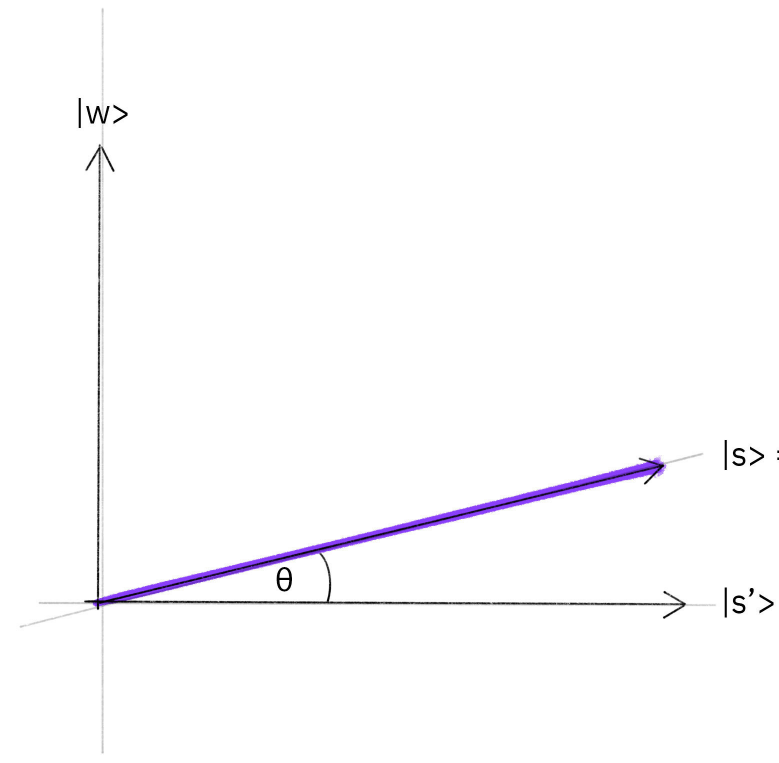
\includegraphics[scale=0.4]{img/grover1.png}
\end{figure}
gdje kut $\theta$ opisuje koliko je stanje $\ket{s}$ zakrenuto prema $\ket{w}$. Za njega vrijedi:
\[
\braket{s|w} = \frac{1}{\sqrt{N}} = \sin\theta \approx \theta
\]

Idući korak algoritma primjenjuje kvantni prorok $U_f$ na stanje $\ket{s}$. Sve što $U_f$ radi jest refleksiju oko stanja $\ket{s'}$:

\begin{figure}[H]
\centering
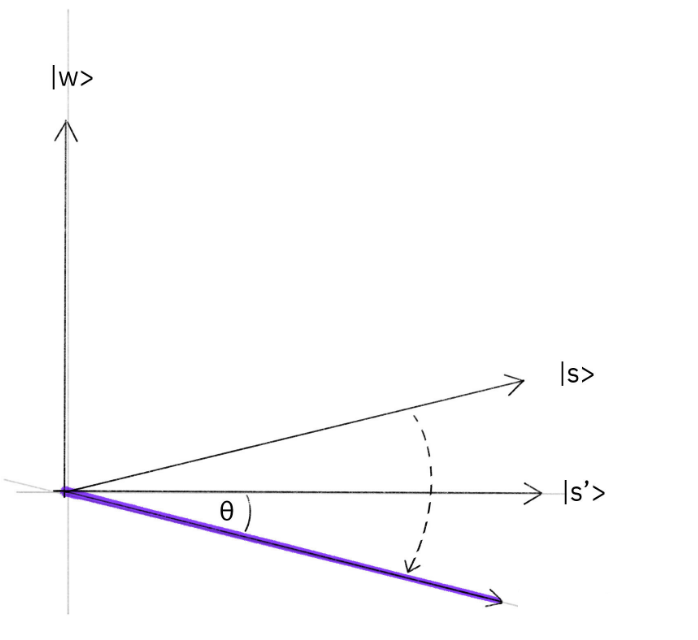
\includegraphics[scale=0.4]{img/grover2.png}
\end{figure}

Zatim se primjenjuje difuzer $U_s$ koji radi refleksiju oko stanja $\ket{s}$:

\begin{figure}[H]
\centering
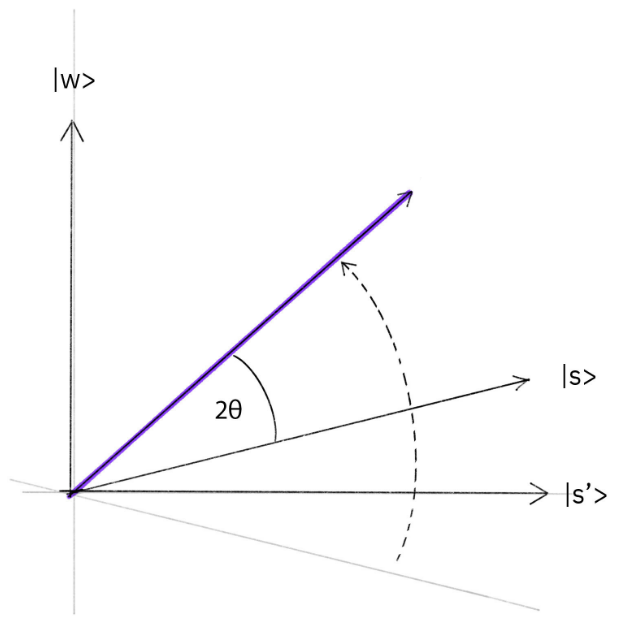
\includegraphics[scale=0.4]{img/grover3.png}
\end{figure}

Dakle, nakon jedne primjene Groverovog operatora, stanje $\ket{s}$ se zaokrenulo za dodatnih $2\theta$ prema ciljnom stanju $\ket{w}$. Nakon $k$ primjena Groverovog operatora, stanje $\ket{s}$ biti će za $(2k + 1)\theta$ zaokrenuto prema stanju $\ket{w}$. Cilj je da to bude što bliže stanju $\ket{w}$, dakle da vrijedi:
\[
(2k + 1)\theta \approx \frac{\pi}{2}
\]
Rješavajući jednadžbu za $k$, dobiva se:
\[
k \approx \frac{\pi}{4\theta} \approx \frac{\pi}{4}\sqrt{N} \approx \sqrt{N}
\]
što znači da je potrebno primijeniti Groverov operator približno $\sqrt{N}$ puta kako bi vjerojatnost mjerenja stanja $\ket{w}$ bila najveća.

\subsection{Kvantni prorok}

Neka je $U_f$ kvantni prorok Groverovog algoritma koji traži stanje $\ket{10}$. Njegova vrijednost iznosi:
\[
U_f = \begin{bmatrix}
1 & 0 & 0 & 0 \\
0 & 1 & 0 & 0 \\
0 & 0 & -1 & 0 \\
0 & 0 & 0 & 1
\end{bmatrix}
\]

Čini se kao da je za samu izgradnju logičkog kruga odnosno proroka potrebno poznavati rješenje koje tražimo što poništava cijeli smisao Groverovog algoritma. To je donekle i istina; poznavanjem matrične reprezentacije proroka, moguće je odrediti ciljna stanja, ili obratno, za konstrukciju proroka na ovakav način, potrebno je poznavati ciljna stanja. Iz toga slijedi da je Groverov algoritam koristan jedino kada se prorok tretira kao crna kutija ili ako se prorok konstruira na način gdje njegova vrijednost nije očita, ali da i dalje daje ispravan rezultat. Takva konstrukcija proroka postiže se koristeći kvantni paralelizam i phase kickback.

Neka je $f$ kriptografska funkcija sažetka za koju vrijedi $f : \{0, 1\}^n \rightarrow \{0, 1\}^m$ te neka je njoj potrebno pronaći inverz.
\begin{figure}[H]
\centering
\begin{quantikz}
\lstick[wires=3]{n} & \gate[wires=6][2cm]{U_{hash}} & \qw & \qw & \gate[wires=6][2cm]{U_{hash}} & \qw \\
\qw & \qw & \qw & \qw & \qw &\qw \\
\qw & \qw & \qw & \qw & \qw & \qw \\
\lstick[wires=3]{m} & & \qw & \ctrl{3} & \qw & \qw \\
\qw &  & \gate{X} & \ctrl{2} & \qw & \qw \\
\qw & & \qw & \ctrl{1} & \qw & \qw \\
\lstick{$\ket{-}$} & \qw & \qw & \targ{} & \qw  & \qw
\end{quantikz}
\caption{Kvantni prorok za pronalaženje inverza od $\ket{101}$}
\end{figure}
Za implementaciju kvantnog proroka potrebno je $n + m + 1$ kvantnih bitova od kojih su $m + 1$ pomoćni. Prvih $n$ bitova se očekuje da su u stanju superpozicije, idućih $m$ bitova se postavlja u stanje $\ket{0}$, dok se zadnji bit postavlja u stanje $\ket{-}$. Zatim je potrebno u kvantnom logičkom krugu implementirati samu funkciju $f$ na način da će joj ulaz biti prvih $n$ bitova, a izlaz idućih $m$ bitova. Koristeći Toffolijeva vrata sa $m$ upravljačkih bitova, može se odabrati izlaz funkcije kojemu je potrebno pronaći inverz (na slici je to $f(x) = 101$). Ciljni bit Toffolijevih vrata je poslijednji bit koji je u stanju $\ket{-}$. Svrha Toffolijevih vrata je svakoj komponenti stanja koja rezultira željenim izlazom promijeniti predznak. To radi koristeći phase kickback. Naime, vrijedi:
\[CNOT\ket{0-} = \ket{0-}\]
\[CNOT\ket{1-} = -\ket{1-}\]
Pošto se prorok koristi iterativno u algoritmu, potrebno je vratiti svih $m$ izlaznih kvantnih bitova u stanje nule. Zbog reverzibilnosti svih operatora, potrebno je samo ponovno primijeniti funkciju $f$.

\section{Shorov algoritam}

\subsection{Opis problema}

Shorov algoritam rješava problem faktorizacije velikih brojeva. To je problem na čiju se tešku izračunljivost oslanja veliki dio modernih kriptografskih mehanizama. Dobar primjer toga jest RSA kriptosustav čija se tajnost privatnog ključa temelji na težini računanja Eulerove funkcije koja se može svesti na problem faktorizacije brojeva. Iz algoritma generiranja ključeva i funkcija enkripcije i dekripcije može se vidjeti zašto je to tako.

Algoritam generiranja ključeva:
\begin{enumerate}
\item Generiranje broja $N = p\cdot q$, gdje su $p$ i $q$ veliki slučajno odabrani prosti brojevi
\item Računanje Eulerove funkcije\footnote{Eulerova funkcija računa broj koji opisuje koliko relativno prostih faktora ima neki broj, tj. veličinu raduciranog sustava ostataka, no ovdje važnije svojstvo Eulerove funkcije jest da ako vrijedi $nzd(a, N) = 1$ onda isto vrijedi $a^{\varphi(N)} \equiv 1\mod N$ } $\varphi(N) = (p-1)(q-1)$
\item Odabir proizvoljnog broja $e$ iz reduciranog sustava ostataka modulo $\varphi(N)$
\item Računanje $d = e^{-1}$ u reduciranom sustavu ostataka modulo $\varphi(N)$
\item Javni ključ: pk = (e, N)
\item Privatni ključ: sk = (d, N)
\end{enumerate}

Funkcija enkripcije:
\[
E(m, (e,N)) = m^e \mod N
\]

Funkcija dekripcije:
\[
D(c,(d,N)) = c^d \mod N
\]

Ovo funkcionira jer vrijedi $e\cdot d = 1\mod \varphi(N)$, tj.
\[
D(m^e,(d,N)) = m^{e\cdot d} \mod N = m \mod N
\]

Dakle, kako bi se narušila sigurnost ovakvog sustava potrebno je moći efikasno izračunati proste faktore, odnosno $\varphi(N)$.

\subsection{Kvantna Fourierova transformacija}

Kvantna Fourierova transformacija transformira bazu računanja iz tzv. Z baze (nazvane po osima Blochove sfere) u tzv. X bazu, odnosno iz $\ket{0}$ i $\ket{1}$ u $\ket{+}$ i $\ket{-}$.

\subsection{Kvantna procjena faze}

\subsection{Opis algoritma}





































